\section*{Programm}
Um die Methoden der Threads in einer Realen Situation zu nutzen, habe ich mich entschlossen ein Programm, welches stark von Threads profitieren kann, zu programmieren.  

Ich habe mich für ein Programm eintscheiden, mit dem man ein Bild mit vielen weiteren Bildern rekrieren kann. Es wird demnach ein Mosaik aus Bildern erstellt.

\begin{figure}[h]
    \centering
    
\includegraphics[height=5cm]{images/Source_100x100}
    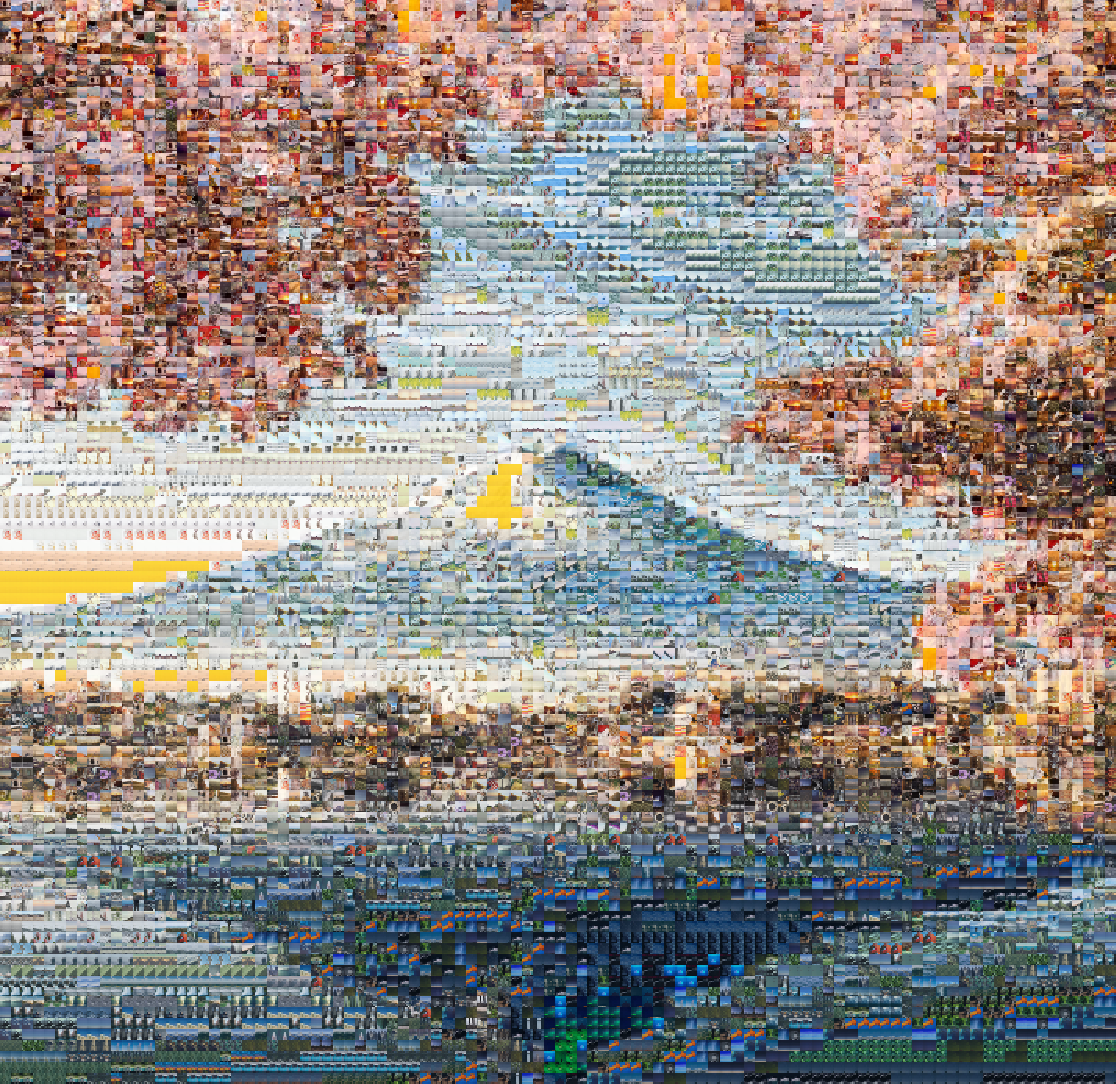
\includegraphics[height=5cm]{images/Render_100x100}
    \caption[Programm Funktion]{Funktionsweise des Programmes}
\end{figure}